
% In order to specifically target the ggF and VBF process, separate analysis categories are defined. The ggF process is analysed in three different regions separated by the number of jets, the VBF process is analysed in one region with at least two jets.  

% Before the specific selections are made in the four individual analysis categories, a common selection is applied to all of them. 

% - Define ``vocabulary'' for regions, bins, categories, processes, ...


Selections are made on event observables to reject as many background events as possible while retaining the majority of the signal events.
A common event preselection is applied before the events are divided into separate analysis \emph{signal regions} (SRs) targeting different signal categories.

\subsection{Preselection}
\label{subsec:preselection}
As discussed in the previous sections, the analysis selects events with exactly two leptons with different flavor and opposite charge as well as satisfying trigger matching criteria.
The transverse momenta of the leptons must satisfy \ptGT{22}\,GeV and \ptGT{15}\,GeV for the higher-\pT (\emph{leading}) and lower-\pT (\emph{subleading}) lepton, respectively.
To minimise the contamination from both low mass meson resonances as well as di-tau backgrounds from low-mass Dell-Yan production, the invariant mass of the dilepton system is required to be $\mll > 10\,\GeV$.
The distribution of the number of jets in the event at the preselection level is shown in \cref{fig:njet-dist}.
The background composition varies significantly across jet bins, which motivates splitting the data sample into separate \Njet categories and further applying specific selection criteria.
In total four mutually exclusive regions are defined.
One region targets the VBF production mode and must satisfy \TwoJet.
Three categories are defined targeting the ggF production mode: \ZeroJet, \OneJet, and \TwoJet.
To exploit the presence of neutrinos in the signal, a minimum threshold criterion of $\pTmiss > 20\,\GeV$ is required for the ggF categories.
To reduce the background contribution from top processes, events are vetoed in all analysis categories if they contain a $b$-jet with \ptGT{20}\,GeV.

% \Cref{subsec:vbf-category,subsec:ggf-zero-jet-category,subsec:ggf-one-jet-category,subsec:ggf-two-jet-category} provide details on the remaining selections used to define the four analysis SRs that are used to measure the ggF and VBF production cross section. A summary of all selections is given in \cref{tab:event-selection}.\todo{Add table}

% The four analysis regions are further split into several kinematic bins according to the Stage-1.2 STXS categorisation scheme, which is described in \cref{subsec:STXS-categorization}.

% cross sections in kinematic fiducial regions defined in the Simplified Template 40 Cross Section (STXS) framework
% that take into account the different event topologies as well as the different background composition.

\subsection{VBF-enriched \TwoJet category}
\label{subsec:vbf-category}
The distinct VBF topology is exploited by rejecting events that contain either an additional jet with \ptGT{30}\,GeV between the two leading jets in pseudorapity (known as \emph{central jet veto} (CJV)) or a lepton at larger pseudorapidities than both of the jets (known as \emph{outside lepton veto} (OLV)).
In addition, a selection is made on the invariant mass of the jets $\mjj > 120\,\GeV$, which mainly serves to separate other physics analyses targeting the $V(\to qq)H$ production mode.
The VBF signal process is then distinguished from the background processes by using a deep neural network model (DNN) that is trained to classify VBF signal and other non-VBF-signal events.
The DNN is used as a final discriminant in the statistical analysis. Details about the development of the VBF DNN analysis are provided in \cref{sec:dnn}.

\todo{Make plot for CJV and OLV}

\subsection{ggF \ZeroJet category}
\label{subsec:ggf-zero-jet-category}
The distinct signal topology arising from the angular momentum correlations explained in \cref{sec:signal-bkg-characteristics} can be best exploited in events with no additional jet.
The opening angle between the missing transverse energy and the dilepton system is required to be $\DPhillMET \,{>}\, 1.57 \approx \frac{\pi}{2}$ and the transverse momentum of the dilepton system is required to have $\Ptll \,{>}\, 30\,\GeV$.
This drastically reduces the amount of background events from DY processes, while retaining a large fraction of signal events.
In addition, the continuum $WW$ production process can be separated from the signal with a requirement of $\mll < 55$\,\GeV\ and the remaining DY background can be further reduced by requiring $\DPhill < 1.8$.
In the statistical analysis, the \ZeroJet SR is further split into four mutually exclusive subregions defined by requiring $\mll \le 30$\,GeV and $\mll > 30$\,GeV, as well as $\pTsublead \le 20$\,GeV and $\pTsublead > 20$\,GeV, where \pTsublead is the \pT of the subleading lepton.
% This $b$-jet veto (or short $b$-veto) in the \ZeroJet\ analysis exploits the energy range below the nominal jet \pT\ threshold of $30\,\GeV$ and reaches down to $\pT = 20\,\GeV$.
% \todo{Reference to the possibility to use track jets?}
\todo{PLOTS}

\subsection{ggF \OneJet category}
\label{subsec:ggf-one-jet-category}
The additional jet in the \OneJet category provides improved rejection against \Ztautau\ processes.
Further reduction of the DY as well as multijet events is achieved with the maximum lepton transverse mass, max($m_{\text{T}}^\ell$), defined as the maximum value of 
\begin{equation}
    m_{\text{T}}^{\ell_i} = \sqrt{ 2 p_\text{T}^{\ell_i} \MET \cdot \left( 1 - \text{cos} \Delta \phi \left( \ell_i, \MET \right) \right) }.
\end{equation}
The max($m_{\text{T}}^\ell$) observable is expected to be smaller for DY and multijet production than for the signal process which motivates a requirement of max($m_{\text{T}}^\ell$)$ > 50\,$GeV.
Another selection is made on the invariant mass of the hypothetical $\tau\tau$ system, $m_{\tau\tau}$.
The $m_{\tau\tau}$ observable is constructed based on the so-called collinear approximation~\cite{PhysRevD.61.093005} that uses the direction and magnitude of the measured missing transverse momentum and projects it along the directions defined by the two reconstructed charged leptons~\cite{PLACEHOLDER:PAPER:CITATION}.
A requirement of $m_{\tau\tau} < m_Z - 25\,\GeV$\footnote{The mass of the $Z$ boson, $m_Z$, is set to the value found in current experimental measurements, 91.1876\,GeV~\cite{PDG2020}.} is applied, which further reduces the contamination of DY processes that tend to have values close to $m_{\tau\tau} = m_Z$.
The same \mll\ and \DPhill\ selections as in the \ZeroJet category are applied in the \OneJet category. As well, the same split into four subregions that is performed in the \ZeroJet category is done in the \OneJet category.
\todo{PLOTS}

\subsection{ggF-enriched \TwoJet category}
\label{subsec:ggf-two-jet-category}
The \TwoJet category targeting the ggF process is made mutually exclusive to the VBF-enriched \TwoJet category by requiring events to fail either the CJV or OLV. 
In addition, events from $V(\to qq) H$ production are highly suppressed by a requirement $|\mjj  - 85| \le 15\,\GeV$ and $\Delta y_{jj} \le 1.2$. 
The same \mll\ and \DPhill\ selections as in the \ZeroJet category are also applied in the ggF-enriched \TwoJet category, and two subregions are defined by a boundary at $\mll = 30\,\GeV$.

\begin{figure}
    \newImageResizeCustom{0.5}{figures/hww/presel/fig_01.pdf}
    \caption{Jet multiplicity distribution for jets with \ptGT{30}\,GeV and \absetaST{4.5}, after applying the preselection criteria including pre-fit normalization. The various background components are discussed in more detail in the text. Previously published in \ccite{ATLAS-CONF-2021-014}.}
    \label{fig:njet-dist}
\end{figure}


\subsection{STXS categorisation}
\label{subsec:STXS-categorization}

-> ggF is written as ggH
-> VBF is denoted as EW qqH that is more inclusive than VBF as it also includes V(->qq)H.

- STXS categorisation plot
- Expected event yields in each stxs region (or maybe later!?)


%%%%% From PAPER

\todo{ALL 1to1 COPIED FROM PAPER FOR NOW. Add citation or re-phrase (vote for citation)}

In order to optimize the measurements in bins aligned with those of the Stage-1.2 STXS framework, several STXS kinematic fiducial regions are merged and the separation of the selected events into SRs differs slightly from the description above.
The STXS bin merging strategy, referred to as Reduced Stage-1.2, and the reconstructed SRs are illustrated in Figure~\ref{fig:STXS_Diagram}.
% \begin{figure}[!h]
%   \centering
%     \includegraphics[width=0.99\textwidth]{figures/hww/}
%   \caption{
%     Two sets (Production Mode Stage and Reduced Stage 1.2) of exclusive phase-space regions (production bins) defined at parton level for the measurement of the Higgs boson production cross sections (left and middle-left shaded panels), and the corresponding reconstructed signal regions (right panel).
%     The description of the production bins as well as the corresponding reconstructed signal regions is given in Section~\ref{sec:STXS-Categorization}.
%     The colors of each reconstructed signal region box indicate the STXS bin which provides the largest relative contribution.
%     \label{fig:STXS_Diagram}
%   }
% \end{figure}
For the exclusive \ZeroJet $ggH$ category, only a single STXS cross section is measured, with the same SR splitting as defined in Section~\ref{sec:ZeroJetCategory} and applying a $\pTH < 200~\GeV$ selection.
For the exclusive \OneJet $ggH$ category, all three Stage-1.2 measurements are retained, with the SR split along the same \pTH bin boundaries.
For the exclusive \TwoJet $ggH$ category with $\pTH < 200~\GeV$, only a single STXS cross section is measured, with the same SR splitting as defined in Section~\ref{sec:ggF-TwoJetCategory} but also including a $\pTH < 200~\GeV$ selection.
For the \Njets inclusive $ggH$ category with $\pTH \ge200~\GeV$, only a single STXS cross section is measured, using both the \OneJet SR with an added $\pTH \ge200~\GeV$ selection and the same ggF-enriched \TwoJet SR with splitting as defined in Section~\ref{sec:ggF-TwoJetCategory} but also including a $\pTH \ge200~\GeV$ selection. No events with \ZeroJet at the event-generation level are reconstructed in the region with $\pTH \ge200~\GeV$.
For the exclusive \TwoJet EW $qqH$ categories targeting VBF production, the bins separated by \pTHjj value\footnote{\pTHjj is defined at the reconstruction level as the transverse momentum of the system composed of the two leptons + \met + two leading jets in the event.} are merged and so are the bins separated by \mjj for $\pTH \ge200~\GeV$, resulting in a total of five measured cross sections.
The same SR described in Section~\ref{sec:VBF-TwoJetCategory} is used, but split into five subregions with the same boundaries that define the measured EW $qqH$ STXS cross sections. In addition, the same DNN and training is used for the final fit's discriminating variable.
The exclusive \TwoJet EW $qqH$ category with $\mjj < 350~\GeV$ that targets $V(\rightarrow q\bar{q})H$ production, and also the $V(\to \textrm{leptons})H$ and $t\bar{t}H$ categories to which this analysis is not sensitive, are fixed to their expected yields in the fit.
Figure~\ref{fig:STXS_Composition} shows the relative contributions of the different merged STXS bins in all reconstructed SRs.
In each case, the target categories provide the largest contribution in the corresponding SRs which aim to select them.

% at the reconstruction level -> using reconstructed objects?

% \begin{figure}[!h]
%   \centering
%     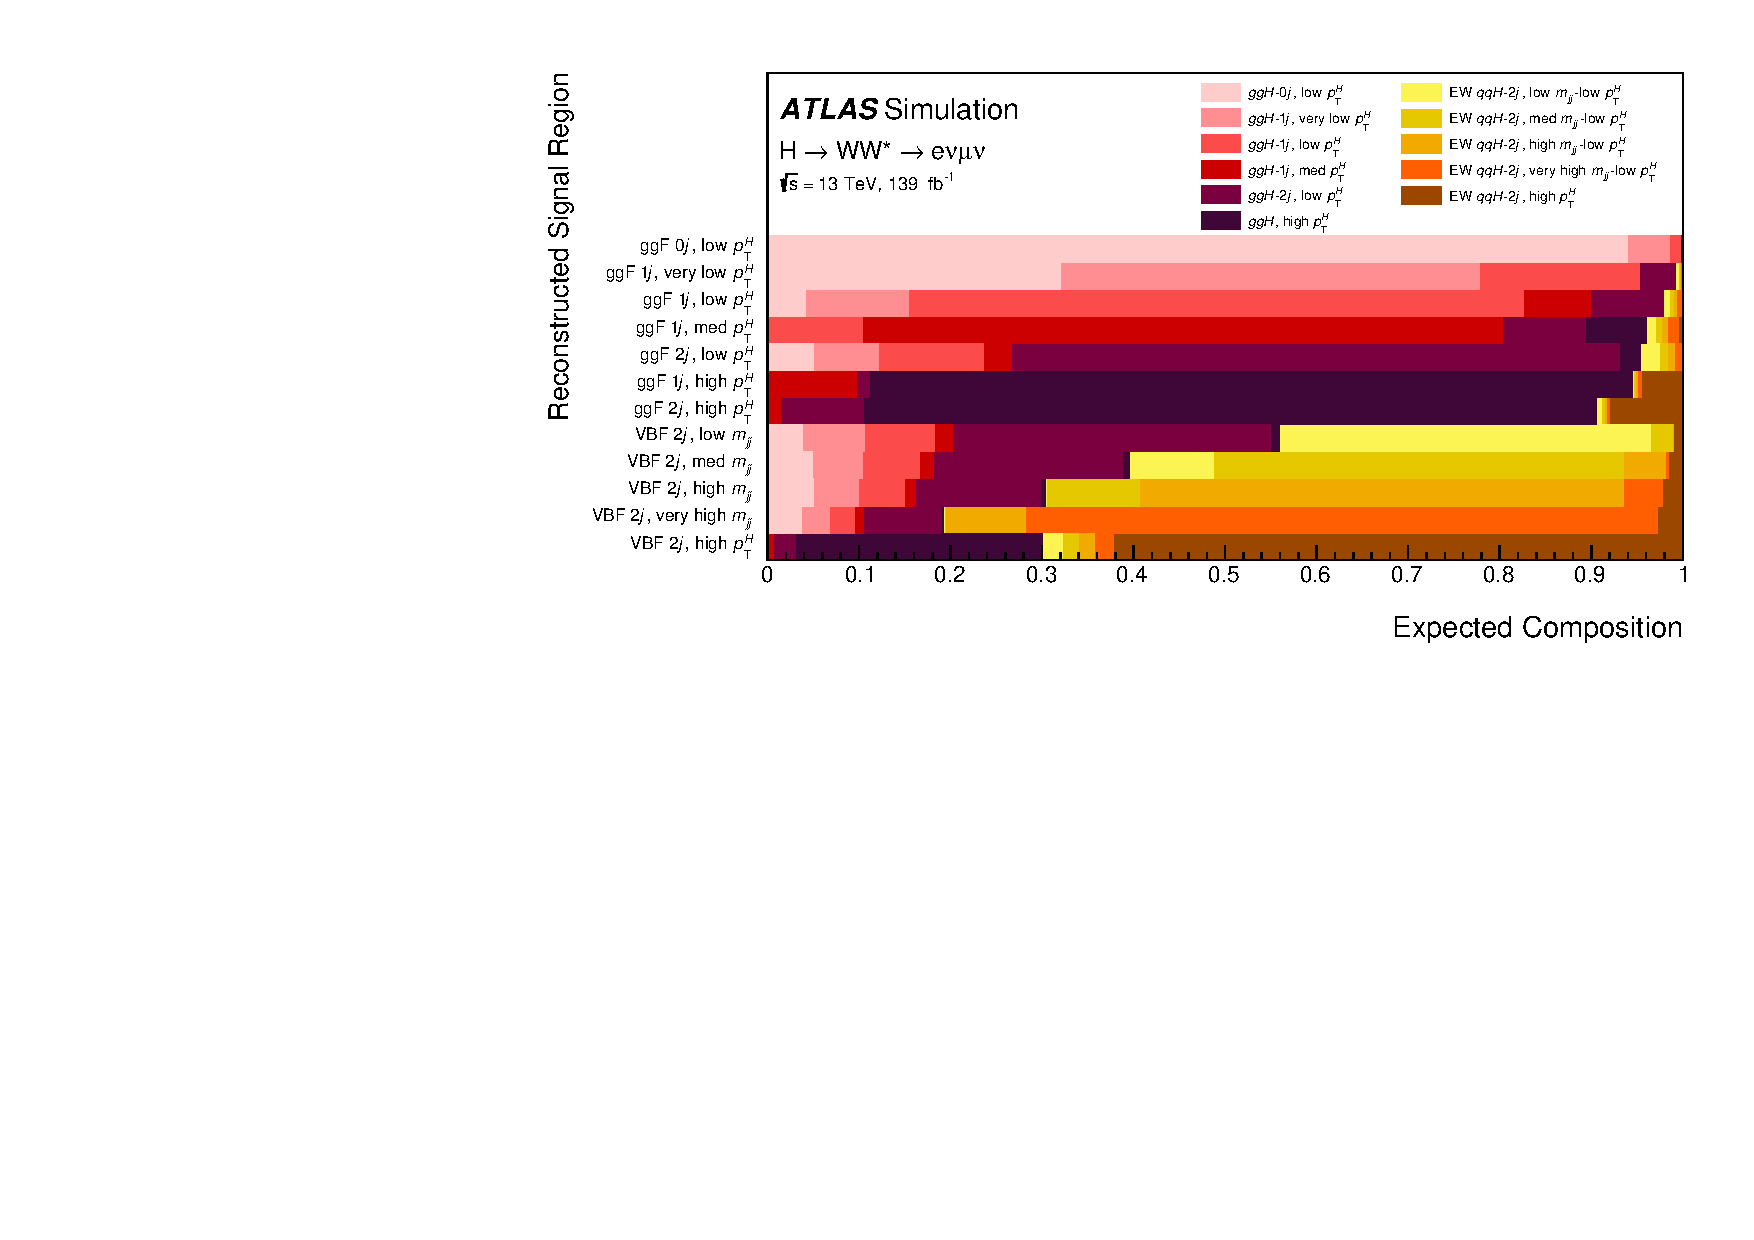
\includegraphics[width=0.90\textwidth]{figures/11-POI/STXS_CompositionMap}
%   \caption{
%     Relative SM signal composition in terms of the measured STXS bin for each reconstructed signal region.
%     \label{fig:STXS_Composition}
%   }
% \end{figure}
